\section{eo\-Binary\-Quality\-Indicator$<$ EOFitness $>$ Class Template Reference}
\label{classeoBinaryQualityIndicator}\index{eoBinaryQualityIndicator@{eoBinaryQualityIndicator}}
Functor Binary quality indicator Binary performance measure to use in the replacement selection process of IBEA (Indicator-Based Evolutionary Algorithm) Of course, EOFitness needs to be an {\bf eo\-Pareto\-Fitness} object.  


{\tt \#include $<$eo\-Binary\-Quality\-Indicator.h$>$}

Inheritance diagram for eo\-Binary\-Quality\-Indicator$<$ EOFitness $>$::\begin{figure}[H]
\begin{center}
\leavevmode
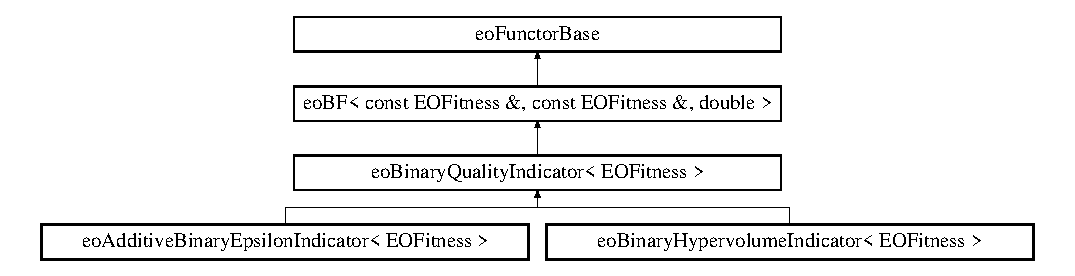
\includegraphics[height=3.25581cm]{classeoBinaryQualityIndicator}
\end{center}
\end{figure}
\subsection*{Public Member Functions}
\begin{CompactItemize}
\item 
{\bf eo\-Binary\-Quality\-Indicator} ()\label{classeoBinaryQualityIndicator_e138f133fb4a5024b2e31f1544b4739a}

\begin{CompactList}\small\item\em constructor \item\end{CompactList}\item 
void {\bf set\-Bounds} (const unsigned \_\-i\-Obj, const double \_\-min, const double \_\-max)
\begin{CompactList}\small\item\em set the bounds for objective \_\-i\-Obj \item\end{CompactList}\end{CompactItemize}
\subsection*{Protected Attributes}
\begin{CompactItemize}
\item 
std::vector$<$ {\bf Range} $>$ {\bf bounds}\label{classeoBinaryQualityIndicator_aa9bb224ab744a00271577a10518581a}

\begin{CompactList}\small\item\em range (min and max double value) for each objective \item\end{CompactList}\end{CompactItemize}
\subsection*{Private Types}
\begin{CompactItemize}
\item 
typedef EOFitness::fitness\_\-traits {\bf traits}\label{classeoBinaryQualityIndicator_3d9415cfa63d3dd57fe44f9e11df3cac}

\begin{CompactList}\small\item\em fitness traits \item\end{CompactList}\end{CompactItemize}
\subsection*{Classes}
\begin{CompactItemize}
\item 
class {\bf Range}
\begin{CompactList}\small\item\em Private class to represent the bounds. \item\end{CompactList}\end{CompactItemize}


\subsection{Detailed Description}
\subsubsection*{template$<$class EOFitness$>$ class eo\-Binary\-Quality\-Indicator$<$ EOFitness $>$}

Functor Binary quality indicator Binary performance measure to use in the replacement selection process of IBEA (Indicator-Based Evolutionary Algorithm) Of course, EOFitness needs to be an {\bf eo\-Pareto\-Fitness} object. 



Definition at line 39 of file eo\-Binary\-Quality\-Indicator.h.

\subsection{Member Function Documentation}
\index{eoBinaryQualityIndicator@{eo\-Binary\-Quality\-Indicator}!setBounds@{setBounds}}
\index{setBounds@{setBounds}!eoBinaryQualityIndicator@{eo\-Binary\-Quality\-Indicator}}
\subsubsection{\setlength{\rightskip}{0pt plus 5cm}template$<$class EOFitness$>$ void {\bf eo\-Binary\-Quality\-Indicator}$<$ EOFitness $>$::set\-Bounds (const unsigned {\em \_\-i\-Obj}, const double {\em \_\-min}, const double {\em \_\-max})\hspace{0.3cm}{\tt  [inline]}}\label{classeoBinaryQualityIndicator_ed08c328526eb4c1c8cfde8b6938ece9}


set the bounds for objective \_\-i\-Obj 

\begin{Desc}
\item[Parameters:]
\begin{description}
\item[{\em unsigned}]\_\-i\-Obj the index of the objective \item[{\em double}]\_\-min the minimum value \item[{\em double}]\_\-max the maximum value \end{description}
\end{Desc}


Definition at line 62 of file eo\-Binary\-Quality\-Indicator.h.

The documentation for this class was generated from the following file:\begin{CompactItemize}
\item 
eo\-Binary\-Quality\-Indicator.h\end{CompactItemize}
